\documentclass[journal]{./IEEE/IEEEtran}
\usepackage{cite,graphicx}

\newcommand{\SPTITLE}{Text Prediction using Probability Matrices and Prefix Trees}
\newcommand{\ADVISEE}{John Alvin L. Sayson}
\newcommand{\ADVISER}{Fermin Roberto G. Lapitan}

\newcommand{\BSCS}{Bachelor of Science in Computer Science}
\newcommand{\ICS}{Institute of Computer Science}
\newcommand{\UPLB}{University of the Philippines Los Ba\~{n}os}
\newcommand{\REMARK}{\thanks{Presented to the Faculty of the \ICS, \UPLB\
                             in partial fulfillment of the requirements
                             for the Degree of \BSCS}}
        
\markboth{CMSC 190 Special Problem, \ICS}{}
\title{\SPTITLE}
\author{\ADVISEE~and~\ADVISER
\REMARK
}
\pubid{\copyright~2019~ICS \UPLB}

%%%%%%%%%%%%%%%%%%%%%%%%%%%%%%%%%%%%%%%%%%%%%%%%%%%%%%%%%%%%%%%%%%%%%%%%%%

\begin{document}

% TITLE
\maketitle

% ABSTRACT
\begin{abstract}
With the advent of the digital age, communication has evolved to a point where technology is seamlessly integrated into day-to-day conversation. Primarily found in mobile phones, text prediction systems involves streamlining the communication by providing users with suggested words that they can select, based on the previous word they provided. This study aims to implement a similar technology, embedded in an application developed for the Chrome browser to provide the power of text prediction in desktop environments, in an application most users use in their day-to-day lives. The predictor was developed using two main and two minor text representations of the text input, of which is the probability matrix, the prefix tree, the sequence, and the bag-of-words respectively.
\end{abstract}

% INDEX TERMS
\begin{keywords}
text generation, text prediction, probability matrices, prefix trees
\end{keywords}

% INTRODUCTION
\section{Introduction}
%Since its conception, literature has served as the backbone of human history, documenting various events that transpired in the past. Throughout the years, however, literature became a creative outlet, bringing forth various books and stories that defined multiple generations.

Verbal communication was always been a vital component of human interaction. After all, it allows two people to be able to understand each other. With the influx and rapid growth of technology over the previous decades, new methods of communication in the digital age were conceived over that timespan.

%It has always been humans that pioneered in creative writing, but in recent years it has become possible for artificial intelligence to write stories of their own, with information obtained from human sources.

Nowadays, prediction keyboards are commonplace in mobile phones. Numerous mobile operating systems seamlessly integrate prediction into the existing keyboard functions to the point where people use it switching from the regular keyboard, to the prediction keyboard, and back again.

It might be common in mobile systems, but what about desktop ones? This study involved investigation on two online applications that provide generated outputs from predefined inputs.

AIWriter\cite{AIWriter} and Botnik's Voicebox are these two applications. AIWriter's process is fully automatic, instantly generating works depending on settings provided by the user in the beginning. On the other hand, Voicebox is more of a hands-on process as the user selects the words suggested by the application in writing their literary works. The suggested words are determined by the source text the user selected in the beginning, ranging from Harry Potter narrations to pancake recipes. If the selection range does not interest the user, they can provide their own source texts by uploading it to the website.

Both website applications improve writing time by doing away with manual word-for-word typing, providing either words or complete paragraphs for the users to use right away. This study intends to provide a similar convenience.

%writing time...
%cite Text prediction systems: a survey here.
Writing or typing time varies from person to person. For those with cognitive, perceptive, and/or physical disabilities, predictive text systems were their preferred medium in being able to communicate easier in social settings. \cite{GV2006} Being able to just use one tap to select words rather than multiple taps per letter, it allows for a great increase in convenience in conversation. As said before, predictive text systems are now embedded in various native keyboards in mobile phones, wherein continuous usage can further personalize the suggested words to the user. Through this, the rate of communication between people can improve. This application aims to achieve a similar goal to that of the common predictive text system. By providing an interface wherein users are given suggestions while in the middle of creating texts, they are able to utilize the power of mobile prediction keyboard functionalities.

%A notable difference from the proposed application from the aforementioned Voicebox is the introduction of genre selection, which eliminates the limit of sticking only to one source material at a time. The mixture of genres produce more varied outputs, and at the same time, more inventive story concepts. 

The application that was implemented as the main output of this study differs from the aforementioned Voicebox is the way the initial input is accepted. The application accepts user input as the initial data for the probability matrix and a prefix tree, which are the two main data structures used for the application.

This paper shall discuss the implementation for the text prediction, as well as the application interface for it.

% OBJECTIVES
\section{Objectives}

\subsection{General Objective}
The study aims to create a text prediction model that utilizes a probability matrix and a prefix tree as its data structures.

\subsection{Specific Objectives}
\begin{enumerate}{\setlabelwidth{1.}}

\item[1.] Receive initial input from the user to instantiate the predictor;

\item[2.] Use the probability matrix data structure in mapping word-level relation;

\item[3.] Use the prefix tree data structure in word prediction;

\item[4.] Present word- and letter-level relation to the end user in the form of a predictive text writer application;

\item[5.] Allow user to create text in the application and allow said text to update the aforementioned data structures; and

\item[6.] Assess the application created using the System Usability Scale.

\end{enumerate}

% RRL
\section{Review of Related Literature}

%\subsection{Previous UPLB and Non-UPLB Works on NLG}

%\subsection{Concept Study of NLG}

%\subsection{Expected Content of RRL}
%\begin{enumerate}{\setlabelwidth{1.}}

%\item[1.]3 Papers Studying Concepts Related to NLG

%\item[2.]7 Papers on Related Studies (UPLB and non-UPLB)

%\item[3.]Applications of Methodologies (based on nos. 1 and 2)

%\end{enumerate}

%ACTUAL CONTENT OF RRL
To understand the possible applications and previous implementations of story and text generation, previous works in the field were observed.

%\subsection{Previous Advances in Text and Literary Work Generation}
%Online Works
%Text Generation from Keywords
Uchimoto, et al. presented various text-generation models in their paper wherein Japanese sentences are formed by feeding the program keywords which serve as the subjects of the sentence it produces. \cite{UKIHSS2002} 
%Discuss some of the language models...

A table of input-output pairs were provided by the authors, with inputs being words in groups of threes and the outputs being complete sentences. From this, a possible limitation provided by their application was that it could only accept three inputs at a time.

\pubidadjcol
The authors have mentioned that the program was created for speakers that are not as fluent in Japanese be able to express sentences that they intend to speak but only know the main words that they want to express. This shows that text generation is not limited to recreational applications, and can be used for accessibility and elaboration. %continue...

%Chinese Poetry Generation with Recurrent Neural Networks
X. Zhang and M. Lapata utilized recurrent neural networks in 2014 to generate Chinese poetry, which follows a specific format for it to be considered one.
\cite{ZXLM2014}
The Chinese poems that they generated follow the quatrain format, wherein four lines of poetry must have five or seven characters each.
The poetry generator functions similarly to Uchimoto's 2002 paper where keywords are accepted to outline the poem's main concept.
In creating the first line, a language model is used to rank candidates that satisfies criteria defined by the poetry format. Following lines are then based on the previous lines. This will ensure continuity from the first line to the last.

%Hierarchal Neural Story Generation
%A paper written by A. Fan, et al. in 2018 used generated sentence prompts that influences the resulting output.

Text generation has also ventured into literary fields with less constraints, specifically story writing.

In 2018, A. Fan, et al. added sentence prompt generation (aside from the expected story generation component) which was then based on to create the corresponding stories. \cite{FLD2018} These prompts are created using a convolutional language model, which contains a novel gated self-attention mechanism created by some of the authors. \cite{DFAG2016}
They also used a sequence-to-sequence network, a model that uses two recurrent neural networks as encoders and decoders, to generate the story based on the prompts trained on the convolutional language model. The sequence-to-sequence model depended upon the trained prompts from the convolutional language model, resulting in a fusion model, as referred to by the writers.

Results shown in the paper contained comparisons between the fusion model and another language model,  presenting the former's readability and higher quality of output over the latter. However, the authors mentioned that one of the limitations of the fusion model is the genericness of the prompts generated, compared to human prompts. This limits the results that can be generated as more specific and varied prompts can provide better results.

%THEORETICAL FRAMEWORK
%\section{Theoretical Framework}

% METHODOLOGY
\section {Methodology}
%\subsection{Expected Content of Methodology}
%\begin{enumerate}{\setlabelwidth{1.}}

%\item[1.]Model for the application

%\item[2.]Details about prototype (backend content)

%\item[3.]Initial results

%\end{enumerate}

%ACTUAL METHODOLOGY
This section contains the features of the implementation of the predictive text application, as well as the evaluation procedures that follow thereafter.

\subsection{Application Implementation}
The application was implemented using only JavaScript, along with the Chrome Extension API to integrate the application with the browser.

\subsection{Prediction Model Visualization}

\begin{figure}[!ht]
\begin{center}

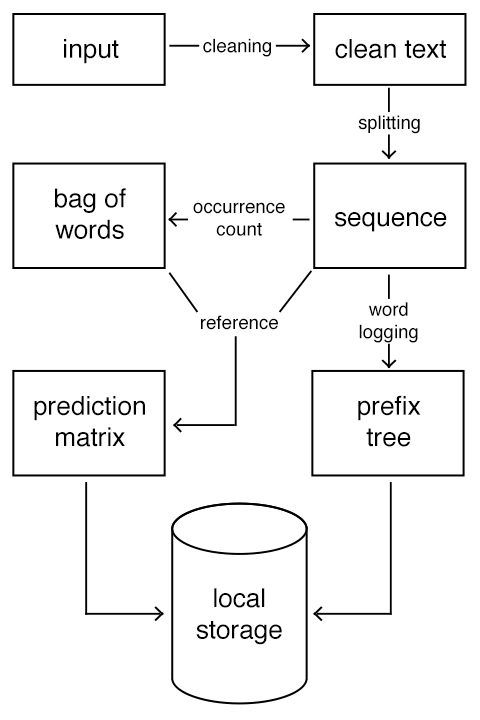
\includegraphics[width=65mm]{images/model.jpg}
\caption{The model used in implementing the predictor.}

\end{center}
\end{figure}

Fig. 1 illustrates the model used in the application, which shall be explained in the following sections.

\subsection{Text Input Representations}
\subsubsection{Sequence}
The sequence is a simple array of strings from the input text, split by a single space (" ") delimiter.

\subsubsection{Bag-of-Words}
The bag-of-words then uses this sequence to count word occurrences.

\subsubsection{Probability Matrix}
The probability matrix uses both previously mentioned representations to produce the probability of a word to appear given another word. This is represented as the matrix keys, which is obtained from the keys of the bag-of-words.

\subsubsection{Prefix Tree}
The prefix tree uses the sequence representation to create the network of letters.

\subsection{Program Flow}
\subsubsection{Input}
Upon installation of the extension, preliminary input data is accepted in a HTML page where the user is asked to enter it. The prefix tree is also loaded with the top 100 common words (according to the Oxford English Corpus) \cite{OxfordFacts}, along with the words provided by the user.

\subsubsection{Processing}
Upon selection of the [Begin Predicting] button in the page for the newly-installed extension, these words are then converted into the four representations mentioned earlier.

The created matrix and prefix tree is stored on the local storage of the browser. The bag-of-words and sequence representations are stored inside the matrix as reference.

Before producing these representations of the text, the text is first cleaned in order to remove various characters and long spaces, which is vital for creating the sequence.

When the user clicks on the [Copy to Clipboard] button on the Text Entry page, the new input is converted into the four representations like in the page for the newly-installed extension. However, instead of directly storing it in the local storage, the application retrieves the saved matrix and prefix tree and merges it with the new ones.

\subsubsection{Output}
While typing in the available text box in the Text Entry Page, the caret location in said text box is used in determining the level of prediction for the next word. If the previously typed word has a space after it, it performs word-level prediction. Else, it performs letter-level prediction.

Word-level prediction uses the matrix, which is why it was important to use the words that appeared in the inputs as the keys. Letter-level prediction uses the prefix tree.

Determining results from the letter-level prediction is just navigating the tree for each letter of the word to be searched and then adding all results from that point onward into an array.

For word-level prediction, the class NameProbabilityPair is used in arranging the most probable words by percentage. Determining the values for the NameProbabilityPair is defined using the equation from the Bayes' theorem, where A is the word to generate possible outputs from, and B is one of the candidate words:
$$ P(A \mid B) = \frac{P(B \mid A) \, P(A)}{P(B)} $$

Meanwhile, the probability of a word is given by this equation:
$$ P(A) = \frac{count(A)}{count(total)} $$

The product of the two are then divided by the probability of B, obtained the same way as A.

The results from these predictions are displayed on the area below the text box, the number which is defined by the user in Settings (default is 6).

\section{Results and Discussion}
This section shall discuss the resulting interface, as well as the evaluation results.

\subsection{Interface}
The application consists of three main screens, the New Predictor screen, the Text Entry screen, and the Settings screen.

\subsubsection{New Predictor}
This screen appears when the extension is installed or upon reset of the predictor.

\begin{figure}[!ht]
\begin{center}

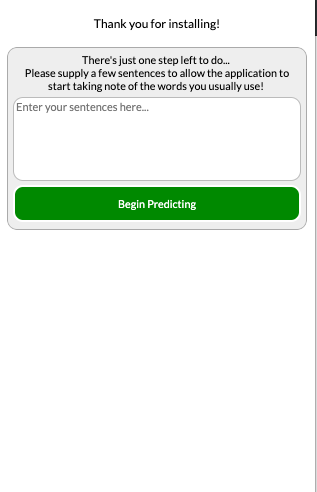
\includegraphics[width=65mm]{images/initial-input.png}
\caption{The New Predictor screen with input posted.}

\end{center}
\end{figure}

\subsubsection{Text Entry}
This screen appears when the extension is installed. This also appears upon reset of the predictor.

\begin{figure}[!ht]
\begin{center}

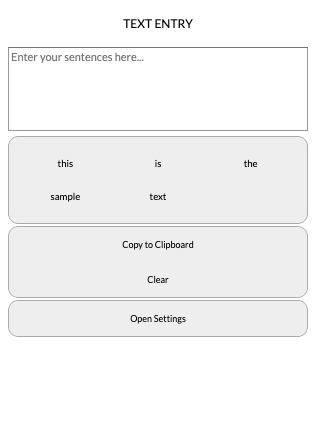
\includegraphics[width=65mm]{images/initial-text-entry.png}
\caption{The Text Entry screen with posted results based off of the input in the previous screen.}

\end{center}
\end{figure}

Fig. 3 illustrates the word-level prediction for the previous input, which is the word "this".

\begin{figure}[!ht]
\begin{center}

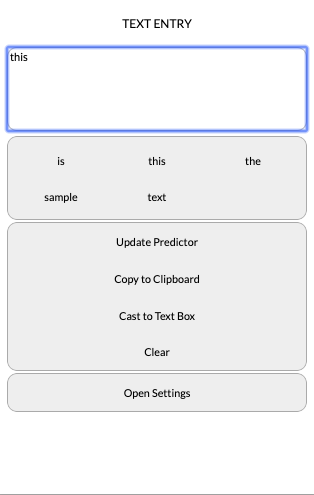
\includegraphics[width=65mm]{images/word-level-prediction.png}
\caption{Word-level prediction functionality.}

\end{center}
\end{figure}

Fig. 4 showcases the letter-level prediction functionality in the application with the input "a". 

\begin{figure}[!ht]
\begin{center}

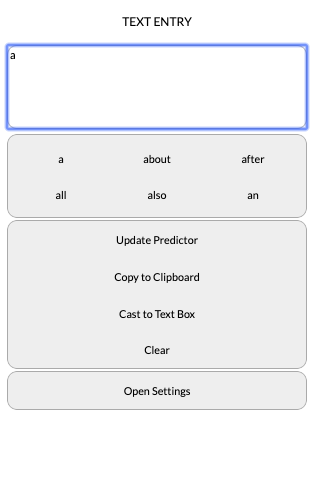
\includegraphics[width=65mm]{images/letter-level-prediction.png}
\caption{Letter-level prediction functionality.}

\end{center}
\end{figure}

\subsubsection{Settings}
Clicking the Open Settings button loads this screen. This contains the setting of the number of keywords, as well as the option to reset the application to its default settings with an empty matrix, prefix tree, etc.

\begin{figure}[!ht]
\begin{center}

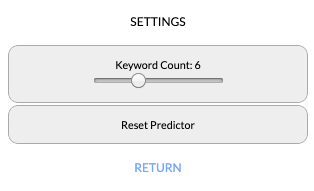
\includegraphics[width=65mm]{images/settings.png}
\caption{The Settings screen.}

\end{center}
\end{figure}

\subsection{Application Evaluation}
The application was evaluated through a survey, using the System Usability Scale as a guide (with small modifications for the statements to fit the context of the study). The respondents were to rate the statements provided by the survey from a 1-5, where 1 means that they completely disagree with the statement and 5 for the opposite.

The application provided for testing consists of two versions. One version of the application is only preloaded with the previously mentioned top 100 words in the English language, and the other was preloaded with a passage of the book \textit{Harry Potter and the Philosopher's Stone}. This was done in order to compare user satisfaction from a newly installed version of the application versus another version where it simulates the performance of the application when it has been used for a longer time. These versions shall be called S (for small) and L (for large), respectively.

These are the survey questions that quantified how much the testers agree with the statements based from the System Usability Scale\cite{UsabilityGeeks}:

\begin{enumerate}{\setlabelwidth{1.}}

\item[1.] I think that I would like to use the application frequently.

\item[2.] I found the application unnecessarily complex.

\item[3.] I thought the application was easy to use.

\item[4.] I think that I would need the support of a technical person to be able to use this application.

\item[5.] I found the various functions in this application were well integrated.

\item[6.] I thought there was too much inconsistency in this application.

\item[7.] I would imagine that most people would learn to use this application very quickly.

\item[8.] I found the application very cumbersome to use.

\item[9.] I felt very confident using the application.

\item[10.] I needed to learn a lot of things before I could get going with this application.

\end{enumerate}

Two questions not derived from the System Usability Scale's template were added to evaluate the user's perceived accuracy of the word- and letter-level prediction functionality of the application.

\begin{enumerate}{\setlabelwidth{1.}}

\item[11.] I think that the word-level prediction for the application provides me with results I expect to appear.

\item[12.] I think that the letter-level prediction for the application provides me with results I expect to appear.

\end{enumerate}

Twenty people selected at random tested the program and submitted their responses to the survey. Before using the guidelines of the System Usability Scale in computing the application score, the weighted average amount for each statement was computed. The resulting score of the L version was 78.375, while the S version had a score of 76.875. According to the System Usability Scale, these scores are close to a grade of A (which is a score of 80.3). 

Based on the provided scores, the L version is preferred by the testers, presumably due to the larger set of words that the application has from the beginning.

The scores 


It is worth noting that the S version scored higher than the L version, despite the SUS evaluation providing the opposite result. A possible cause for this result is that the S version provides a smaller set of data, decreasing the amount of words that the testers expect to appear.

% CONCLUSION AND FUTURE WORK
\section{Conclusion and Future Work}
This study involves the development of a text prediction model implemented using a probability matrix and a prefix tree, as well as sequences and bag-of-words. This model was then used to develop an application as an extension for the Chrome browser similar to prediction keyboard systems commonly found in mobile phones.

Through user evaluation, the application was shown to have performed satisfactorily both in its usability as well as the perceived accuracy of the testers involved in the study.
%The application produced was able to perform predictions both in the letter-level and the word-level, implemented using four representations of the text input. Upon evaluation, the application performs favorably under most conditions.

%However, during the evaluation through surveys, the comments stated that the user interface needed some work regarding text sizes and design consistency. Considering as the overall user experience received the least evaluation of 3.9, further enhancements to this component should be observed. Some comments also suggested the possibility of preloading a huge dataset of words into the prefix tree in order.

%Some comments also considered using this kind of application for making predictions using tweets as an input, which would involve data mining for scraping tweets.

% BIBLIOGRAPHY
\bibliographystyle{./IEEE/IEEEtran}
\bibliography{./sayson-cs190-ieee}
\nocite{*}

% BIOGRAPHY
\begin{biography}
[{
\includegraphics{images/sayson.jpg}}]
{John Alvin L. Sayson} is an undergraduate student of the University of the Philippines Los Ba\~{n}os. He likes to spend the day sleeping, playing music games and occasionally using his trusty keyboard to play music.
\end{biography}


\end{document}
 
